\documentclass{intcov_report}
\usepackage{blindtext}

\usepackage{float}
\title{Description of Datasets and Usage}

\begin{document}

\setcounter{page}{1}

\maketitle

\section{Possible targets and deliverables}

Developing a smart city platform with the goals in the user requirements report would involve several specific goals and subprojects. Here are some example tasks\footnote{WOI=working on it}:

\begin{enumerate}

\item Traffic Management:

 \begin{itemize}
  \item [WOI] Real-time traffic monitoring and analysis to identify congestion hotspots.
   \item [WOI] Predictive modeling for traffic flow optimization and proactive management.
   \item Intelligent traffic signal control to optimize signal timings based on current traffic conditions.
   \item Route optimization and dynamic rerouting to minimize travel time and congestion.
 \end{itemize}
 
 \item Weather Prediction:
 
  \begin{itemize}
   \item Accurate weather forecasting using advanced AI algorithms.
   \item [WOI] Integration of weather data with the smart city platform to provide real-time weather information.
   \item Proactive alert systems to notify citizens and officials about severe weather conditions.
   \item [WOI] Predictive modeling to assess the impact of weather on various aspects of the city, such as transportation and infrastructure.
   \end{itemize}

 \item Pedestrian Movement Analysis:
 
   \begin{itemize}
   \item [WOI] Utilizing computer vision and AI technologies to analyze pedestrian movement patterns.
   \item Identifying pedestrian-heavy areas to optimize urban planning and transportation infrastructure.
   \item Real-time monitoring and analysis to improve pedestrian safety and optimize pedestrian flows.
   \item Integration with public transportation systems to enhance multimodal transportation options.
   \end{itemize}


\item Public Safety:

   \begin{itemize}
   \item Integrating surveillance cameras with computer vision algorithms for real-time threat detection.
   \item [WOI] Developing AI-based systems to identify and respond to incidents such as accidents, crimes, and emergencies.
   \item Enhancing emergency response capabilities through real-time data analysis and predictive modeling.
   \item Implementing smart lighting and video analytics for improved safety in public spaces.
   \end{itemize}

\item Urban Planning and Sustainability:

   \begin{itemize}
   \item Analyzing historical and real-time data to optimize urban planning decisions.
   \item Developing models for efficient resource allocation, such as energy and water management.
   \item Promoting sustainable practices by encouraging the use of electric vehicles and renewable energy sources.
   \item Creating interactive platforms to engage citizens in urban planning processes and gather feedback.
   \end{itemize}

\end{enumerate}


 
\section{Current tasks}

\subsection{Real-time traffic monitoring and analysis to identify congestion hotspots}

Apply prediction of total number of vehicles at Tanah Merah Coast Rd (Camera 1113, (1.317036,103.988598)) in front of Tanah Merah Ferry Terminal. 


\subparagraph{Flowchart}

\begin{enumerate}
\item Fetch images every 5min 
\item Detect objects in each image with deep learning YOLOv7 model.
     \begin{figure}[H]
         \centering
         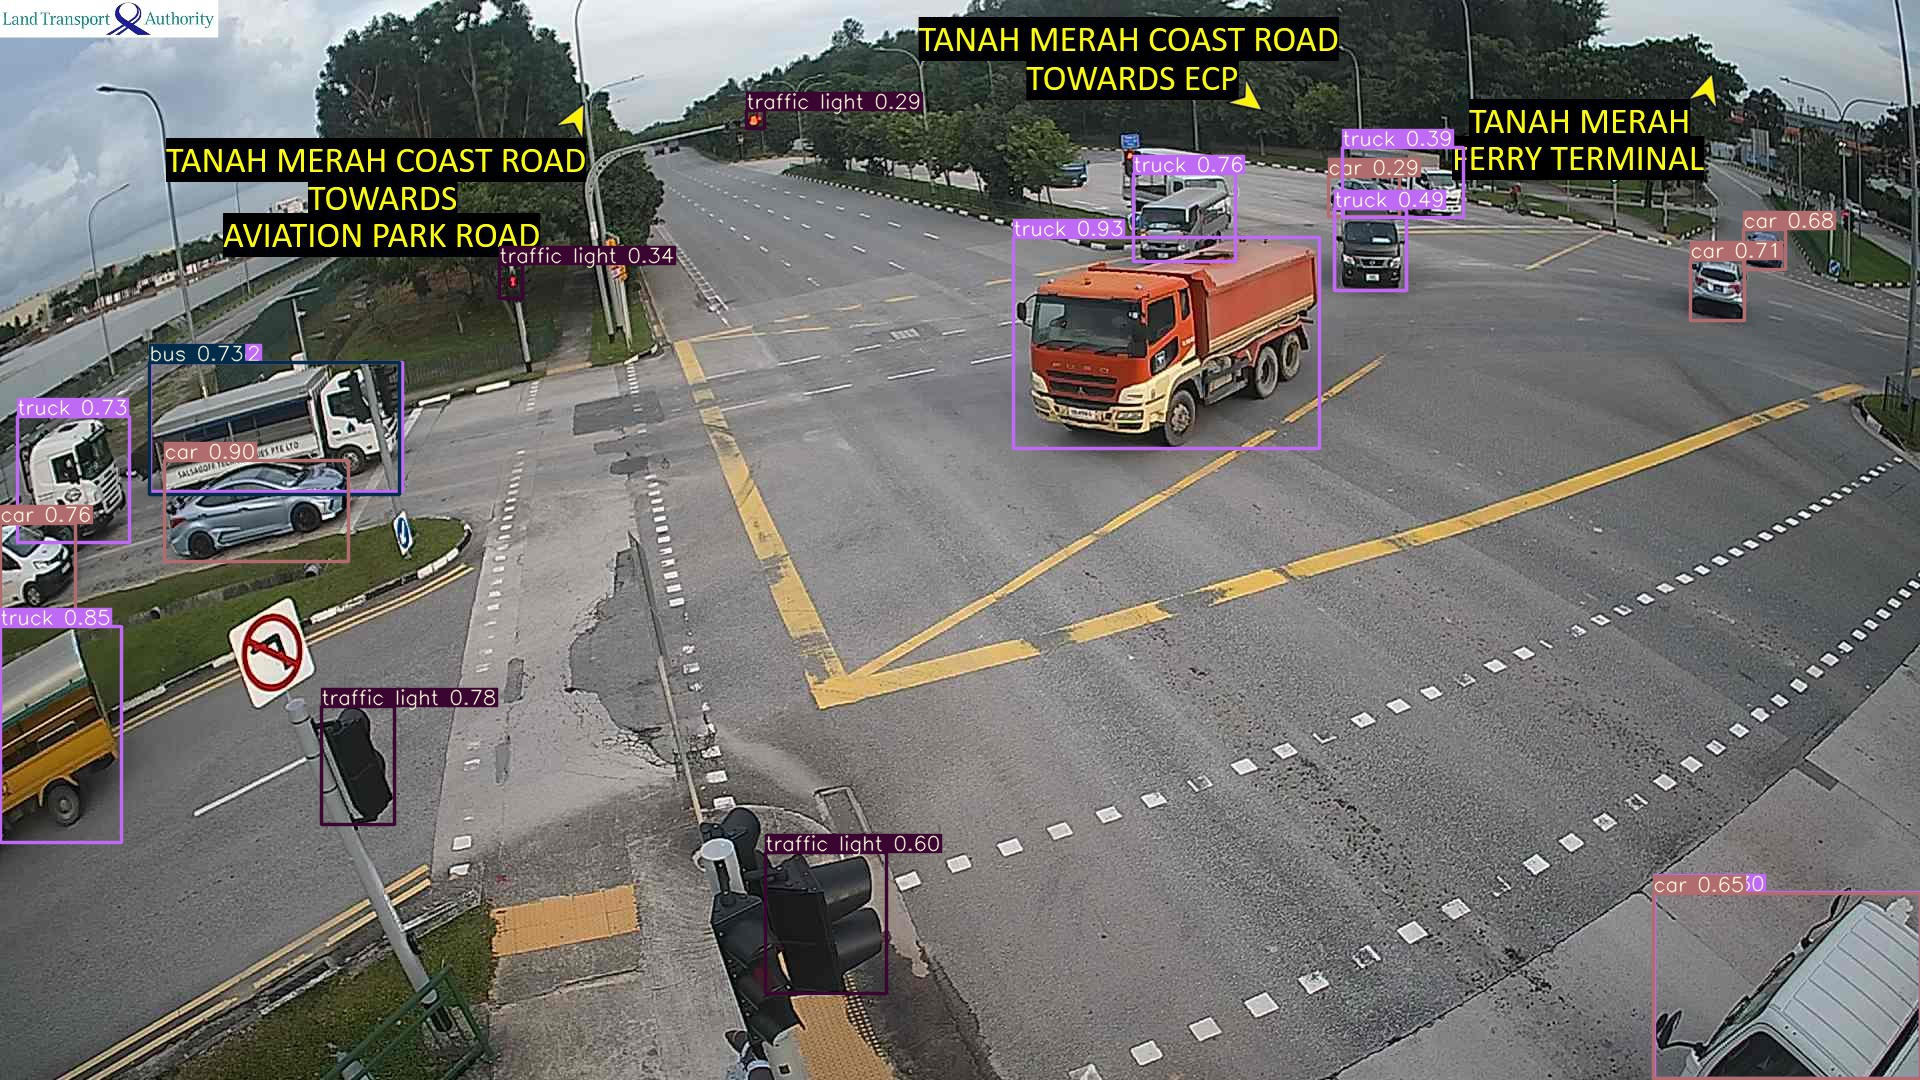
\includegraphics[width=\textwidth]{vehicle_detection.jpg}
         \label{fig:vehicle_detection}
         \caption{Example of object detection}
     \end{figure}
     
\item Select objects ['bicycle', 'bus', 'car', 'motorcycle', 'person', 'truck']
\item Count TotalVehicles and TotalPedestrians 
     \begin{figure}[H]
         \centering
         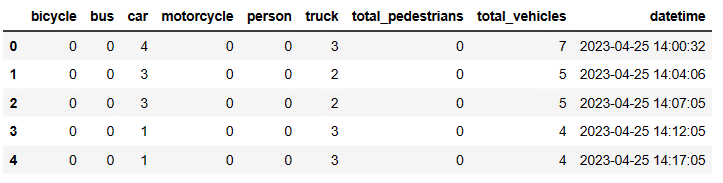
\includegraphics[width=0.8\textwidth]{vehicle_number_table.png}
         \label{fig:vehicle_number_table}
         \caption{Example of data table}
     \end{figure}

\item Use moving average for low level prediction 

     \begin{figure}[H]
         \centering
         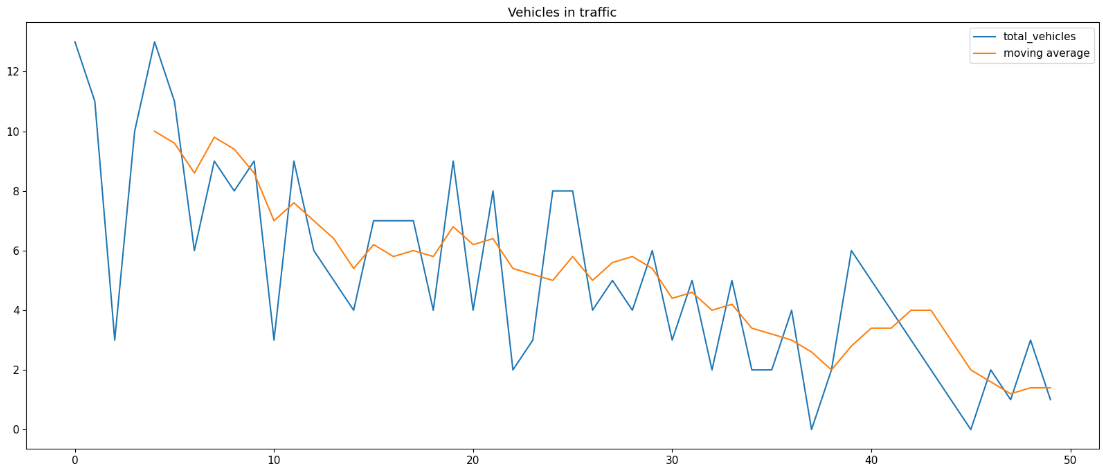
\includegraphics[width=0.8\textwidth]{prediction_moving_avg.png}
         \label{fig:prediction_moving_avg}
         \caption{Prediction using moving average}
     \end{figure}
  
\item Use statistical models with lookback on historical data to predict TotalVehicles in the next few minutes (prediction with ARIMA models results in unbounded results, so we show only first few predictions after observation point zero).

     \begin{figure}[H]
         \centering
         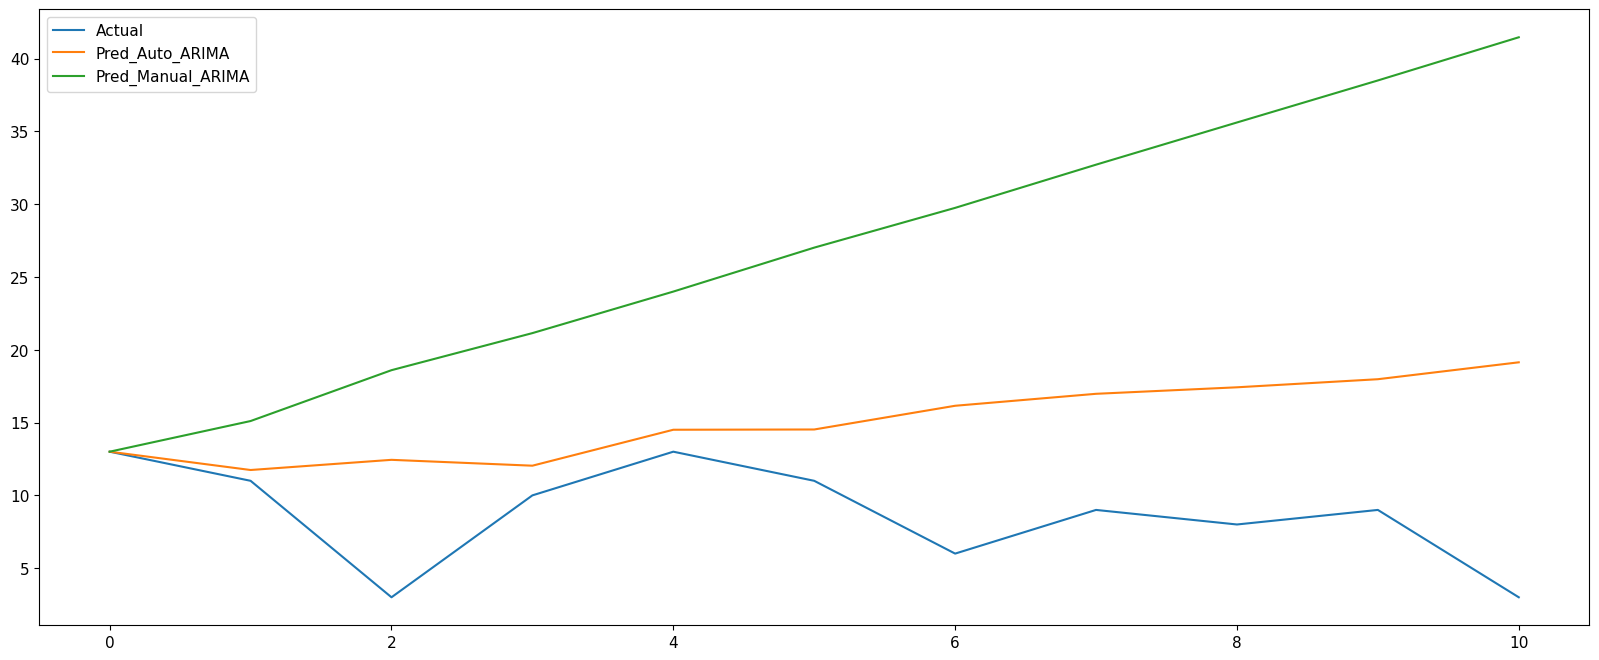
\includegraphics[width=0.8\textwidth]{prediction_arima.png}
         \label{fig:prediction_arima}
         \caption{Prediction using ARIMA statistical models}
     \end{figure}
   
\item Use an AI machine learning LSTM model (lookback for the 5 previous images namely last 5*5=25minutes) to predict TotalVehicles in the next 5 minutes

     \begin{figure}[H]
         \centering
         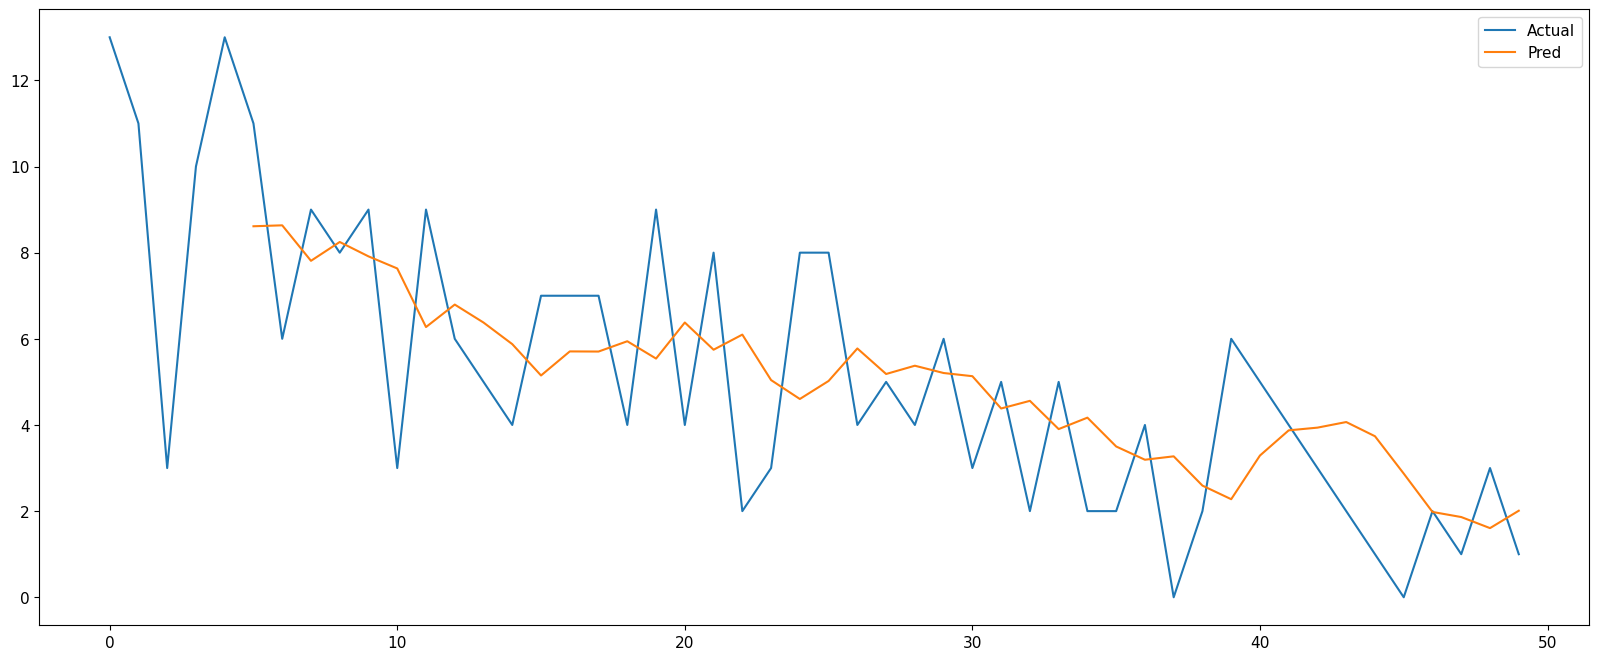
\includegraphics[width=0.8\textwidth]{prediction_lstm.png}
         \label{fig:prediction_lstm}
         \caption{Prediction using LSTM machine learning model}
     \end{figure}
     
\item Evaluate models in terms of error performance

\begin{table}[H]
\caption{Error results for vehicle number prediction}

\begin{center}
\begin{tabular}{ l c c c c } 
 \hline
 Method & MSE & RMSE & MAE & MAPE \\
  \hline
Moving average & 3.133043 & 1.770041 & 1.526087 & 4.503600e+14\\
Manual ARIMA & 454.584526 & 21.320988 & 18.263936 & 3.193929\\
Auto ARIMA & 64.102944 & 8.006431 & 6.356743 & 1.271673\\
LSTM & 4.518527 & 2.125683 & 1.828363 & 6.148179e+14\\

 \hline
\end{tabular}
 \\Note: Errors are better when smaller.\\
 MSE = Mean Squared Error \\
 RMSE = Root Mean Squared Error\\
 MAE = Mean Absolute Error\\
 MAPE = Mean Absolute Percentage Error
\end{center}
\label{tab:vehicle_pred_results}

\end{table}


\end{enumerate}

\subparagraph{Issues}
\begin{itemize}
\item Misclassification of objects as in \autoref{fig:misclasified} e.g. \\

2023-05-04 07:25:45: {'person': 3, 'car': 2, 'airplane': 2, 'truck': 5, 'traffic light': 5}
2023-05-09 20:46:46: {'car': 1, 'airplane': 1, 'bus': 1, 'truck': 1, 'traffic light': 8}


\begin{figure}[H]
     \centering
     \begin{subfigure}[b]{0.45\textwidth}
         \centering
         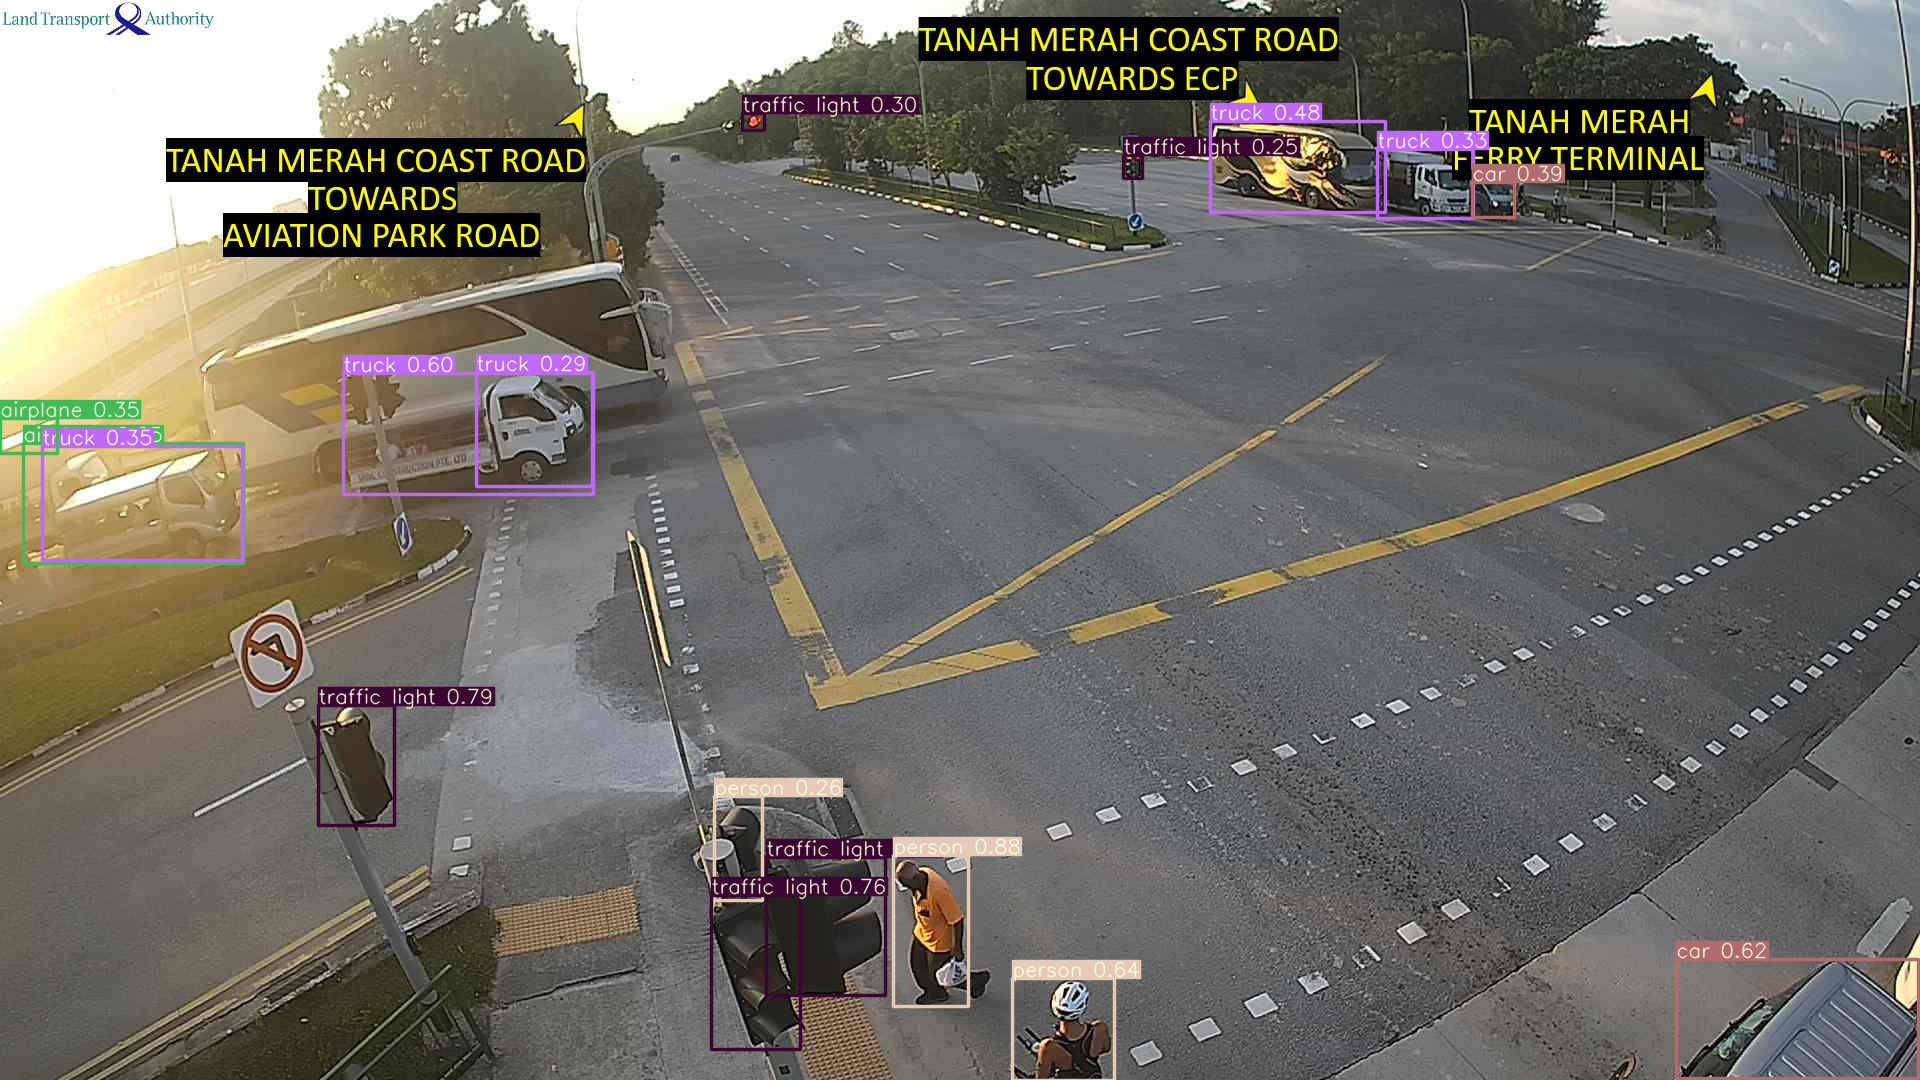
\includegraphics[width=\textwidth]{airplane_1.png}
         \caption{2023-05-04 07:25:45}
     \end{subfigure}
     \hfill
     \begin{subfigure}[b]{0.45\textwidth}
         \centering
         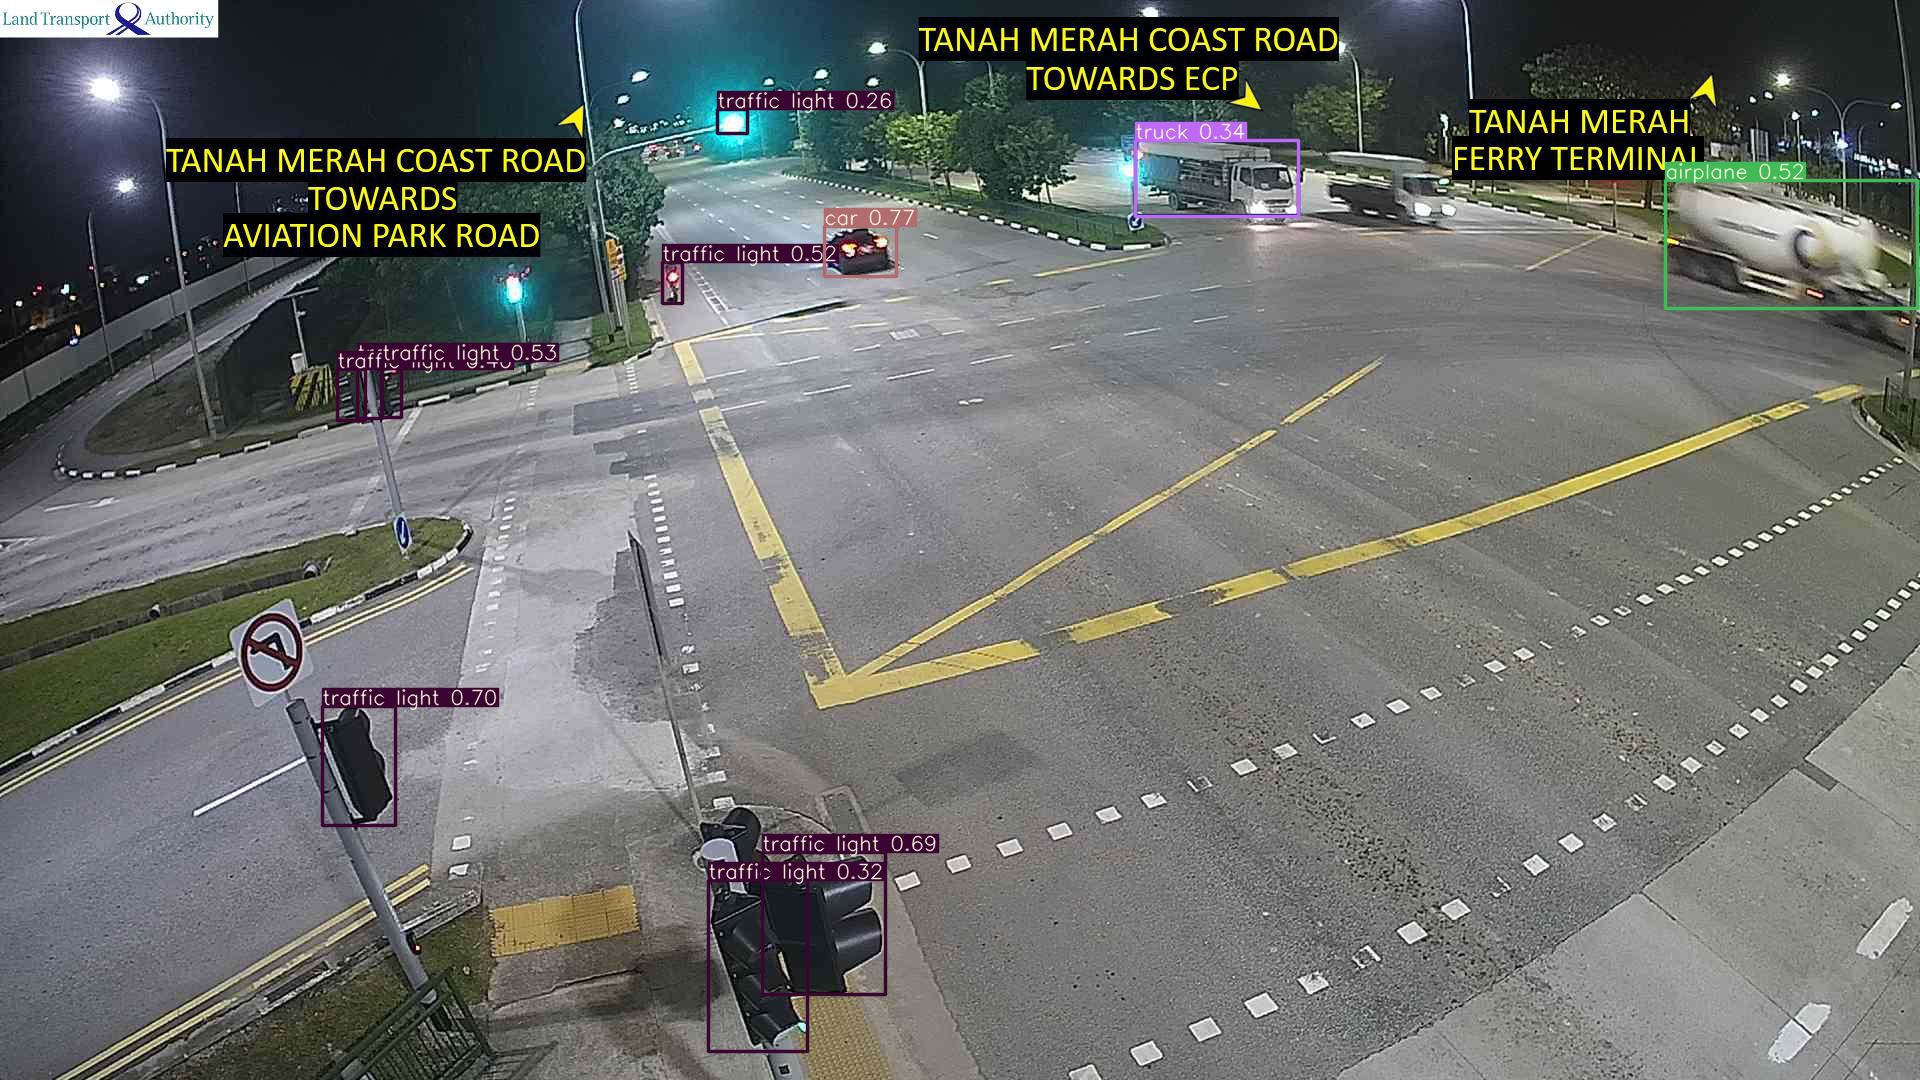
\includegraphics[width=\textwidth]{airplane_2.png}
         \caption{2023-05-09 20:46:46}
     \end{subfigure}
     \caption{Example: false detection of airplanes on the highway}
        \label{fig:misclasified}
\end{figure}

\end{itemize}

\subparagraph{Conclusions\\}
The number of vehicles in the train set is affected by the number of misdetections of the YOLOv7 model. Therefore, the quality of the training dataset is reduced. ARIMA-based statistical model underperform in this case. The simple moving average and the complex LSTM have similar performance in vehicle number prediction.


\end{document}
